\chapter{Глава 2 (проектирование)}
Будем рассматривать табличный метод синтеза. Для начала потребуется таблица отсчётов, чтобы её вычислить используем готовый инструмент.
	
	\begin{figure}[H]
    \centering
    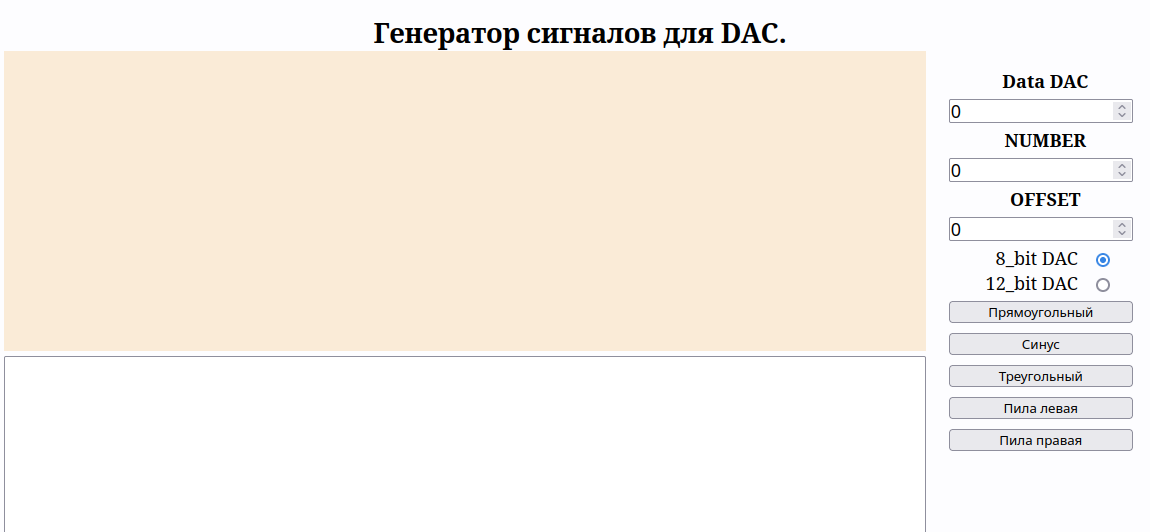
\includegraphics[width=1\textwidth]{../image/lut_prog.png}
    \caption{Программа для вычисления значений сигнала.}
	\end{figure}
	
	У таблицы есть 4 параметра:
	\begin{enumerate}
		\item Разрядность ЦАП: 8 или 12 бит.
		\item Максимальное значение.
		\item Количество значений.
		\item Смещение от нуля.
	\end{enumerate}
	
	Использовать мы будем 12-битные значения в количестве 256 чисел. Максимальное значение амплитуды сигнала может быть 4095, но так как для улучшения генерации будет задействован встроенный в цифро-аналоговый преобразователь выходной буфер, то он будет срезать сигнал сверху и снизу на 0.2В, поэтому значения тоже следует срезать на эту же величину для корректной генерации.
	
	В документе от ST про работу с цифро-аналоговым преобразователем есть формула для расчета выходного напряжения.
	
	$DAC_{output} = V_{REF}*\dfrac{DOR}{DAC_{MaxDigitalValue} + 1}$, где DOR --- цифровое значение.
	
	Нам нужно найти какое значение соответствует напряжению 0.2В. Выразим DOR и подставим имеющиеся значения.
	
	$DOR = \dfrac{V_{REF}}{DOR}*DAC_{MaxDigitalValue} + 1 = \dfrac{3.3}{0.2}*(4095+1) = 248$
	
	Укажем смещение от нуля 248, а максимальное значение 4095 меньше на 248, то есть 3847 и сгенеририуем таблицу отсчётов для синусоиды. 
	
	\begin{figure}[H]
    \centering
    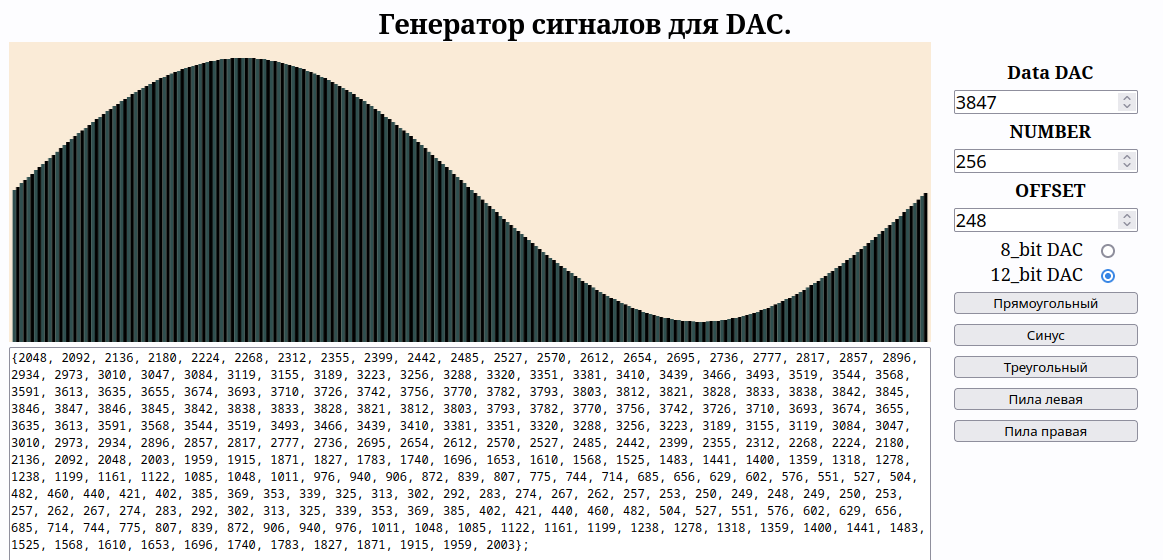
\includegraphics[width=1\textwidth]{../image/lut.png}
    \caption{Вычисление таблицы сигнала.}
	\end{figure}
	
	Теперь у нас есть данные для генерации сигнала, но теперь нужно продумать как передавать их в цап и как вообще работать с цапом.
%\section{Моделирование прямого цифрового синтеза}

Смоделируем алгоритм метода прямого цифрового синтеза на языке Си для дальнейшей реализации на микроконтроллере.

\begin{code}
\captionof{listing}{Метод DDS.}
\begin{minted}[mathescape,linenos,frame=lines,breaklines]{text}
int main() {
  uint16_t p_acc, p_step;
  uint8_t addr = 0; // адрес ячейки

  p_acc = 0;    // аккумулятор фазы
  p_step = 128; // код частоты

  while(1)
  {
    addr = p_acc >> 8; // выделение старшей части аккумулятора фазы
    p_acc += p_step;   // шаг
    printf("%d 0x%X\n", addr, sinus[addr]); // вывод отсчёта
  }

  return 0;
}
\end{minted}
\end{code}

	
	Код частоты задаёт выходную частоту генератора. При значении 256 вывод будет следующий:
	
\begin{figure}[H]
    \centering
    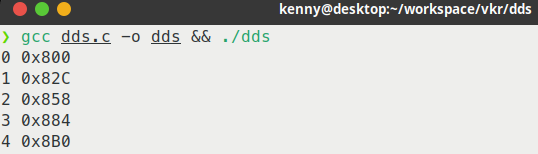
\includegraphics[width=0.6\textwidth]{../image/dds256.png}
    \caption{Формирование отсчётов при коде частоты 256.}
\end{figure}
	
	Увеличим код частоты в два раза и получим следующее:

\begin{figure}[H]
    \centering
    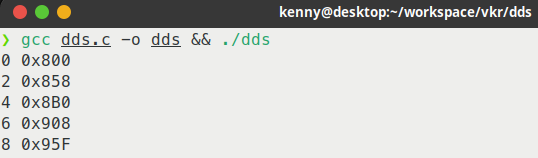
\includegraphics[width=0.6\textwidth]{../image/dds512.png}
    \caption{Формирование отсчётов при коде частоты 512.}
\end{figure}

	Как можно заметить отсчёты стали формироваться через один, соответственно частота вырастит в два раза. Теперь уменьшим частоту в два раза выставив код частоты 128.

\begin{figure}[H]
    \centering
    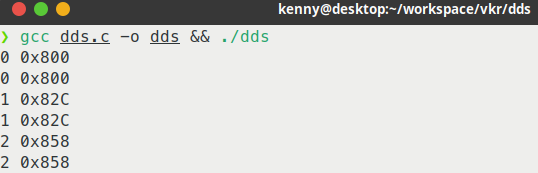
\includegraphics[width=0.6\textwidth]{../image/dds128.png}
    \caption{Формирование отсчётов при коде частоты 128.}
\end{figure}

	Программа стала выводить каждый отсчёт по два раза тем самым, понизив частоту.
	
	В данном виде модуляции код частоты просто абстрактное число, которое добавляется к аккумулятору фазы и узнать реальную частоту проблематично. Результат синтеза будет проверен опытным путём на микроконтроллере.

%\section{Алгоритм работы}


%\section{Схема генератора}
\begin{figure}[h]
    \centering
    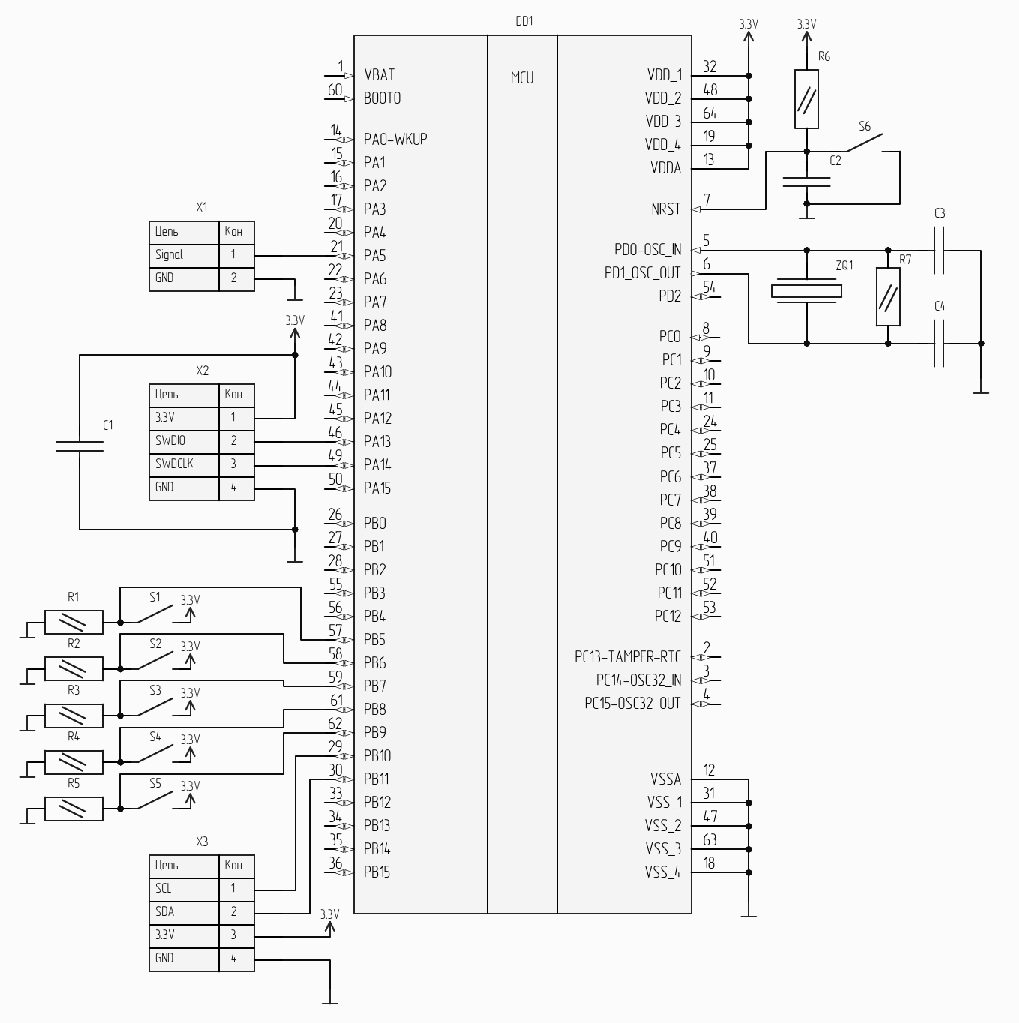
\includegraphics[width=1.0\textwidth]{../image/scheme-cropped.pdf}
    \caption{Схема электрическая принципиальная.}
\end{figure}

\section{Вывод из второй главы}
